\documentclass[10pt,
               a4paper,
               journal,
               ]{IEEEtran}
\makeatletter

\def\markboth#1#2{\def\leftmark{\@IEEEcompsoconly{\sffamily}\MakeUppercase{\protect#1}}%
\def\rightmark{\@IEEEcompsoconly{\sffamily}\MakeUppercase{\protect#2}}}
\makeatother

\usepackage[utf8]{inputenc}
\usepackage[T1]{fontenc}
\usepackage{cite}
\usepackage{amsfonts}
\usepackage[pdftex]{graphicx}
\graphicspath{{../png/}}
\DeclareGraphicsExtensions{.png}
\usepackage[cmex10]{amsmath}
\interdisplaylinepenalty=2500
\usepackage{array}
\usepackage{mdwmath}
\usepackage{mdwtab}
\usepackage{eqparbox}
\usepackage[caption=false,font=footnotesize]{subfig}
\usepackage{fixltx2e}
\usepackage{stfloats}
\usepackage{url}
\hyphenation{op-tical net-works semi-conduc-tor}
\usepackage{stmaryrd}
\usepackage{bbding}
\usepackage{algpseudocode}
\usepackage{algorithm}
\usepackage{tikz}
\usetikzlibrary{shapes}
\usetikzlibrary{calc}
\usetikzlibrary{positioning}
\usepackage{listings}
\usepackage{color}

\definecolor{dkgreen}{rgb}{0,0.6,0}
\definecolor{gray}{rgb}{0.5,0.5,0.5}
\definecolor{mauve}{rgb}{0.58,0,0.82}

\lstset{frame=tb,
  language=C++,
  aboveskip=3mm,
  belowskip=3mm,
  showstringspaces=false,
  columns=flexible,
  basicstyle={\small\ttfamily},
  numbers=none,
  numberstyle=\tiny\color{gray},
  keywordstyle=\color{blue},
  commentstyle=\color{dkgreen},
  stringstyle=\color{mauve},
  breaklines=true,
  breakatwhitespace=true
  tabsize=3
}

\newcommand{\reffig}[1]{{[Fig.~\ref{#1}.]}}
\newcommand{\refeq}[1]{{[Eq.~\ref{#1}.]}}

\begin{document}
	\title{Constraint Programming - Inside Gecode}
	\author{Benedikt~Schmidt}
	\markboth{Advanced Seminar for Security in Information Technology, Summer Term 2014}%
	{Benedikt Schmidt: Constraint Programming - Inside Gecode}	
	\maketitle	
	
	\begin{abstract}	
		\textit{last thing to write}	
	\end{abstract}
	
	\section{Introduction}
	Constraint programming is a tool to solve mathematical problems through the formulation of constraints, which describe the desired solution. As typically a foraml and exact definition, like it can be found in \cite[p.~16]{handbookCP} for constraint propagation, is not as helpful as an example, I would like to give you a short overview on the topic through the well known problem \emph{SEND MORE MONEY}.
	
	Consider the problem
	\[SEND + MORE = MONEY\]
	where every character is a variable and the position in the word describes the weight.
	\begin{equation}
	\label{eq:linearConstraint}
	\begin{split}
		& S \cdot 10^3 + E \cdot 10^2 + N \cdot 10^1 + D \cdot 10^0 + \\ 
		& M \cdot 10^3 + O \cdot 10^2 + R \cdot 10^1 + E \cdot 10^0 = \\ 
		& M \cdot 10^4 + O \cdot 10^3 + N \cdot 10^2 + E \cdot 10^1 + Y \cdot 10^0
	\end{split}
	\end{equation}		
	
	To narrow the solution space a little bit down I state additional constraints:
	\begin{enumerate}
	\item All variables must have different values.
		\begin{equation}
		\begin{split}
			S \ne E \land S \ne N \land & S \ne D \land \dots \land \\
			E \ne N \land & E \ne D \land \dots \land \\
			& N \ne D \land \dots
		\end{split}
		\end{equation}	
	\item There must not be a trailing zero. Combined with the so-called all-different constraint \cite{allDifferent} from above this results in
		\begin{equation}
			S \ne 0 \land M \ne 0
		\end{equation}
	\end{enumerate}
	
	Now a solver for constraint programming like Gecode provides the necessary tools to define these constraints in their most natural form as equations and inequations and will find all possible solutions or just one of them, depending on the selected search algorithm. Actually this example contains only linear constraints and could therefore be solved through linear programming. As linear programming is only a subset of constraint programming the latter one is often the more useful one, because not every problem in the real world is linear or can be linearized in a useful way. Consequently constraint programming with its ability to consider constraints in there most general form can be used in various fields like scheduling of resources, computer-aided design and robotics \cite[p.~221]{trendsInCP}.
	
	In the following I will describe the necessary steps to solve a problem with constraint programming and as example of an implementation I will always refer to \emph{Gecode} \cite{gecode}.
	
	\section{State of the Art}
	\subsection{Variable Domains}
	In constraint programming to a variable a set of possible values is connected, the so called domain. This domain can be a finite or inifite set of integers, true or false and intervals. Depending on the domain a variable is called an integer, boolean or floating variable. Possible ranges for a variable $x$ of each domain are:
	\begin{itemize}
		\item Integer: $x \in \mathbb{N}$, $x \in \{-5, 4, 10\}$, \dots
		\item Bool: $x \in \{\text{true}, \text{false}\}$
		\item Float: $x \in [-4, 3]$, $x \in [-10, 8] \cup [10, 12]$, \dots
	\end{itemize}
	This distinction is important as especially for floating variables the classical approach to constraint programming, a backtrack search, can not be applied directly. For integer and boolean variables the domain for each variable is reduced step by step during a search, either by constraints which rule out certain values or by trial and error. As floating variables do not have discrete values for their domains the procedere in this case is to reduce or split intervals based on constraints or to apply trial and error through splitting the intervals \cite[p.~571]{handbookCP}. I will come back to this topic later during the discussion of the branch-and-bound search.
	
	\subsection{Constraint Types}
	
	\begin{figure}
	\center
	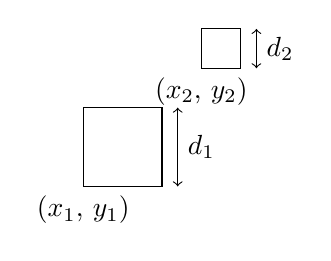
\begin{tikzpicture}
		\draw (0, 0) rectangle (1, 1);
		\node at (0, -0.3) {($x_1$, $y_1$)};
		\draw[arrows=<->] (1.2, 0) -- (1.2, 1);
		\node at (1.5, 0.5) {$d_1$};
		\draw (1.5, 1.5) rectangle(2, 2);
		\node at (1.5, 1.2) {($x_2$, $y_2$)};
		\draw[arrows=<->] (2.2, 1.5) -- (2.2, 2);
		\node at (2.5, 1.75) {$d_2$};
	\end{tikzpicture}
	\caption{two squares which should not overlap}
	\label{fig:squares}
	\end{figure}
	
	As already mentioned before constraint programming is the generalization of linear programming, therefore it is at least possible do define linear constraints like \refeq{eq:linearConstraint}. Which statements are possible to make varies than very much from the programming language in which the problem is implemented and the used toolset. Typical constraints would be
	\begin{itemize}
		\item Equalities: $x = y + 2$, $x^2 + y^2 = 1$, \dots
		\item Inequalities: $x \ne y$, \dots
		\item Relations: $x < 2 y$, $e^x < 4$, \dots
	\end{itemize}
	In Gecode for example it is very easy to create for example a nonlinear constraint based on the integer variables a, b, c and d \cite[p.~120]{programmingGecode}:
	\begin{lstlisting}
rel(home, a+b*(c+d) == 0);
	\end{lstlisting}
	This single statement in C++ implements the constraint
	\begin{equation}
		a + b \cdot (c + d) == 0
	\end{equation}
	which is a quite handy way to do it.
	
	Hence there are boolean variables available it is also possible to use logical operators to combine other constraint types to logical expressions. To show the usage of this on an example I will give the implementation for the placement of two squares such that they do not overlap \reffig{fig:squares}. This problem can be expressed mathematically by \cite[p. 101]{programmingGecode}
	\begin{equation}
	\begin{split}
		x_1 + d_1 \le x_2 & \lor x_2 + d_2 \le x_1 \lor \\
		y_1 + d_1 \le y_2 & \lor y_2 + d_2 \le y_1
	\end{split}
	\end{equation}
	and in Gecode by
	\begin{lstlisting}
rel(home,	(x1 + d1 <= x2) || 
		(x2 + d2 <= x1) || 
		(y1 + d1 <= y2) || 
		(y2 + d2 <= y1));
	\end{lstlisting}
	which is again quite obvious to a reader with some experience in a C-like programming language.	
	
	\subsection{Constraint Propagation}
	Constraint propagation is a key concept in constraint programming as it allows to speed-up the search significantly. The term propagation refers in this area to the reduction of domains of variables which are infeasible, considering other constraints and affected variable domains. As the size of the variable domain is related to possibilities which have to be checked by a search, the constraint propagation is able to prune infeasible subtrees. Therefore the whole search process is accelerated.
	
	\begin{figure}
	\center
	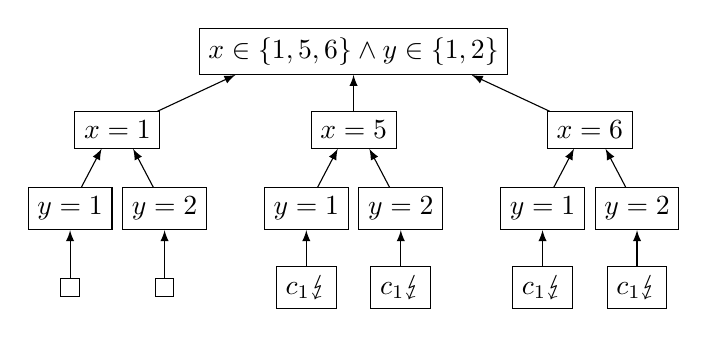
\begin{tikzpicture}
		\tikzstyle{arrow}=[draw, -latex]
		\node[rectangle,draw] at (0, 3) (levelOne) {$x \in \{1, 5, 6\} \land y \in \{1, 2\}$};
		
		\node[rectangle,draw] at (-3, 2) (levelTwoElementOne) {$x = 1$};
		\coordinate[left=1.5cm of levelOne.south] (levelOnePointOne);
  		\path[arrow] (levelTwoElementOne) -- (levelOnePointOne);
  		
		\node[rectangle,draw] at (0, 2) (levelTwoElementTwo) {$x = 5$};
		\coordinate[left=0cm of levelOne.south] (levelOnePointTwo);
  		\path[arrow] (levelTwoElementTwo) -- (levelOnePointTwo);
  		
		\node[rectangle,draw] at (3, 2) (levelTwoElementThree) {$x = 6$};
		\coordinate[right=1.5cm of levelOne.south] (levelOnePointThree);
  		\path[arrow] (levelTwoElementThree) -- (levelOnePointThree);
  		
		\node[rectangle,draw] at (-3.6, 1) (levelThreeElementOne) {$y = 1$};
		\coordinate[left=0.2cm of levelTwoElementOne.south] (levelTwoElementOnePointOne);
  		\path[arrow] (levelThreeElementOne) -- (levelTwoElementOnePointOne);
		\node[rectangle,draw] at (-3.6, 0) (levelFourElementOne) {\Checkmark};
  		\path[arrow] (levelFourElementOne) -- (levelThreeElementOne);
		\node[rectangle,draw] at (-2.4, 1) (levelThreeElementTwo) {$y = 2$};
		\coordinate[right=0.2cm of levelTwoElementOne.south] (levelTwoElementOnePointTwo);
  		\path[arrow] (levelThreeElementTwo) -- (levelTwoElementOnePointTwo);
		\node[rectangle,draw] at (-2.4, 0) (levelFourElementTwo) {\Checkmark};
  		\path[arrow] (levelFourElementTwo) -- (levelThreeElementTwo);
  		
		\node[rectangle,draw] at (-0.6, 1) (levelThreeElementThree) {$y = 1$};
		\coordinate[left=0.2cm of levelTwoElementTwo.south] (levelTwoElementTwoPointOne);
  		\path[arrow] (levelThreeElementThree) -- (levelTwoElementTwoPointOne);
		\node[rectangle,draw] at (-0.6, 0) (levelFourElementThree) {$c_1 \lightning$};
  		\path[arrow] (levelFourElementThree) -- (levelThreeElementThree);
		\node[rectangle,draw] at (0.6, 1) (levelThreeElementFour) {$y = 2$};
		\coordinate[right=0.2cm of levelTwoElementTwo.south] (levelTwoElementTwoPointTwo);
  		\path[arrow] (levelThreeElementFour) -- (levelTwoElementTwoPointTwo);
		\node[rectangle,draw] at (0.6, 0) (levelFourElementFour) {$c_1 \lightning$};
  		\path[arrow] (levelFourElementFour) -- (levelThreeElementFour);
  		
		\node[rectangle,draw] at (2.4, 1) (levelThreeElementFive) {$y = 1$};
		\coordinate[left=0.2cm of levelTwoElementThree.south] (levelTwoElementThreePointOne);
  		\path[arrow] (levelThreeElementFive) -- (levelTwoElementThreePointOne);
		\node[rectangle,draw] at (2.4, 0) (levelFourElementFive) {$c_1 \lightning$};
  		\path[arrow] (levelFourElementFive) -- (levelThreeElementFive);
		\node[rectangle,draw] at (3.6, 1) (levelThreeElementSix) {$y = 2$};
		\coordinate[right=0.2cm of levelTwoElementThree.south] (levelTwoElementThreePointTwo);
  		\path[arrow] (levelThreeElementSix) -- (levelTwoElementThreePointTwo);
		\node[rectangle,draw] at (3.6, 0) (levelFourElementSix) {$c_1 \lightning$};
  		\path[arrow] (levelFourElementSix) -- (levelThreeElementSix);
	\end{tikzpicture}
	\caption{search tree without constraint propagation}
	\label{fig:bigTree}
	\end{figure}
	
	\begin{figure}
	\center
	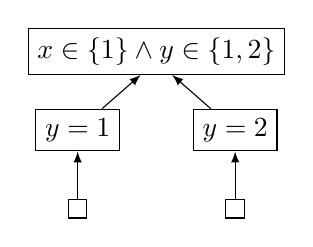
\begin{tikzpicture}
		\tikzstyle{arrow}=[draw, -latex]
		\node[rectangle,draw] at (0, 2) (levelOne) {$x \in \{1\} \land y \in \{1, 2\}$};
  		
		\node[rectangle,draw] at (-1, 1) (levelTwoElementOne) {$y = 1$};
		\coordinate[left=0.2cm of levelOne.south] (levelOnePointOne);
  		\path[arrow] (levelTwoElementOne) -- (levelOnePointOne);
		\node[rectangle,draw] at (-1, 0) (levelThreeElementOne) {\Checkmark};
  		\path[arrow] (levelThreeElementOne) -- (levelTwoElementOne);
		\node[rectangle,draw] at (1, 1) (levelTwoElementTwo) {$y = 2$};
		\coordinate[right=0.2cm of levelOne.south] (levelOnePointTwo);
  		\path[arrow] (levelTwoElementTwo) -- (levelOnePointTwo);
		\node[rectangle,draw] at (1, 0) (levelThreeElementTwo) {\Checkmark};
  		\path[arrow] (levelThreeElementTwo) -- (levelTwoElementTwo);
	\end{tikzpicture}
	\caption{search tree with constraint propagation}
	\label{fig:smallTree}
	\end{figure}
	
	To visualize this effect consider a constraint problem based on two variables $x \in \{1, 5, 6\}$ and $y \in \{1, 2\}$ and one constraint based on them.
	\begin{equation}
		c_1:\ x \le y
	\end{equation}
	Without constraint propagation and branching first on $x$ this results in search tree \reffig{fig:bigTree}. Obviously the right parts of this tree can already be pruned already at the root by propagation of constraint $c_1$ and therefore it is not necessary to create and evaluate these subtrees \reffig{fig:smallTree}.
	
	The actual implementation of constraint propagation differs again from one toolset to another, but the basic concepts are for sure the same. As the topic of this paper is the implementation in Gecode I will concentrate on this one.
	
	Constraints in Gecode are always evaluated ahead of a further growth of a subtree, as it may be possible to prune some of the subtrees. The problem here is to decide in which order the constraints should be considered, and it may even be necessary to evaluate some constraints more often. A short example will explain this very well \cite[p.~575]{handbookCP}: Let there be two constraints 
	\begin{equation}
		c_1: y - x^2 = 0
	\end{equation}
	\begin{equation}
		c_2: y - x - 1 = 0
	\end{equation}
	and let the variable domains be $x, y \in [-4, 4]$. Starting with the evaluation of constraint one follows a chain of reductions of the variable domains, based only on constraint propagation:
	\begin{equation}
	\begin{split}
		c_1:\ &y \in [-4, 4] \rightarrow y \in [0, 4] \\
		c_1:\ &x \in [-4, 4] \rightarrow x \in [-2, 2] \\
		c_2:\ &y \in [0, 4] \rightarrow y \in [0, 3] \\
		c_2:\ &x \in [-2, 2] \rightarrow x \in [-1, 2] \\
		c_1:\ &x \in [-1, 2] \rightarrow x \in [-1, 1.73 \dots] \\
		&\dots
	\end{split}
	\end{equation}
	Actually this behaviour is very nice to have as it narrows efficiently the search space down.
	
	To implement this repeated evaluation of constraints in Gecode all constraints subscribe to the domains of the variables which are part of them. With this method the constraints get noticed whenever a variable domain is reduced and they can signal the system that they need to be evaluated once again.
	
	The next difficult decision is which constraint should be evaluated first. In the example above the constraints were quite simple and therefore it won't make a big difference to evaluate first $c_1$ or $c_2$, the search will take nearly the same time. Unfortunately not all constraints are that easy to evaluate and for this case Gecode defines for every constraint a certain cost \cite[p.~275]{programmingGecode}. Based on this cost the constraints are sorted into buckets which are then iterated from the constraints with lower costs to the ones with higher costs. This means, whenever a variable domain is changed, the first try is to use constraints with the lowest possible cost and only if none of them needs to be evaluated constraints with higher costs are considered.
	
	\subsection{Search Algorithms}
	In constraint programming search algorithm define the way the search tree is constructed, starting from the root node. To improve the performance of the search usually at every newly created node a constraint propagation is executed to narrow the search space down. Based on these two steps then either one, the best or no solution is found. What the actual result in the end is depends obviously on the search algorithm.
	
	In Gecode it is possible to define its own search strategies, but the user is supported at this point with some standard engines which can be used to build custom ones:
	\begin{itemize}
	\item Depth-First Search
	\item Limited Discrepancy Search
	\item Branch-and-Bound Search
	\item Depth-First Search Restart Optimization
	\end{itemize}
	
	In the following part I will discuss these searches and some additional, well known techniques, which can be applied during searches in constraint programming.
	
	\subsubsection{Branching Strategies}
	If at one node it is not possible to empty one variable domain or to reduce all variable domains to the size one it is necessary to make a decision: How should be the next subtree be build? The question is answered by the selected branching strategy, which depends on the variable domain. For Integer (and Bool) Variables there are three possible strategies \cite[p.~87]{handbookCP} which differ in how the domain is distributed to the subtrees. All the strategies have in common that they create additional temporary constraints, which are only valid for the specific subtree. The temporay addition of constraints is called \emph{posting}.
	\begin{itemize}
	\item Enumeration: The domain for $x \in D = {x_1, x_2, \dots}$ is split up into $|D|$-branches where for every branch $i$ one additional constraint $c:\ x = x_i$ is posted.
	\item Binary choice points: One value $x_i$ of the domain $D$ of the variable $x$ is selected and the domain is split up into two subtrees: On one the constraint $x = x_i$ and on the other one the constraint $x \ne x_i$ is posted. This results into something like a binary tree at this point.
	\item Domain splitting: The domain $D$ for the variable $x$ is split up into two disjoint intervals or sets, for example $x < 2$ and $x \ge 2$.
	\end{itemize}
	
	Obviously for variables with a Float domain the Enumeration and Binary choice points are not feasible, but the last one, domain splitting, is typically used. As termination criteria for a Float it is often necessary to define a epsilon which describes the interval length, at which the solver states to have found a solution.
	
	For all branching strategies there is a big choice of freedom left, which can be used to implement some heuristics. This additional information is either gained during the search itself of pre defined by the user.
	
	\subsubsection{Depth-First Search}
	\begin{algorithm}
		\begin{algorithmic}
			\Function{DFS}{node}
				\If{$Goal(node)$}
					\State \Return $node$
				\EndIf
				\State $s \gets Successors(node)$
				\If{$Null(s)$}
					\State \Return $nil$
				\EndIf
				\State $result \gets DFS(Left(s))$
				\If{$result \ne nil$}
					\State \Return $result$
				\Else
					\State \Return $DFS(Right(s))$
				\EndIf
			\EndFunction
		\end{algorithmic}
		\caption{Depth-first search in a binary search tree for one feasible solution, without constraint propagation}
	\end{algorithm}
	
	The Depth-first search is a good point to start, as it was also historical the first developed one. The idea behind this search algorithm is that every possible combination of variables is examined. Obviously in its basic form it can not be applied to problems with inifinite domains; for problems with such variable domains it is necessary to use for example a Branch-and-Bound Search. Sometimes the Depth-First Search is also referred to as chronological backtrack search.
	
	The starting point is the root node, from where one the algorithm is called recursively. At every node mainly two steps are executed: First a constraint propagation and then a branching, which divides the search space into two disjoint sub spaces, on which the same algorithm is applied again. The search stops in a leave if either no branching is possible anymore and therefore a valid solution is found, or one or more variable domains are emptied, which indicates that in this leave no possible solution exists.
	
	This search is a so-called complete algorithm as it can be proven that all possible solutions will be found \cite[p.~85]{handbookCP}. Because of this characteristic it is very useful to proove for example that for a certain problem no solution exists. The main drawback obviously is the execution time, as it does an exhaustive search, and maybe even the memory usage if during the search many solutions are found.
	
	By stopping the search after one feasible solution is found the algorithm the Depth-first search can often be accelerated. Although this slightly modified version is not complete anymore, in practice it is in some areas sufficient to know just one valid solution.
	
	\subsubsection{Depth-First Search with Optimization}
	If in the constraint programming is a certain objective is defined which should be either minimized or maximized a modified version of the Depth-first search can be applied. The only difference is that it evalutes the objective function for every found solution concerning the constraints and stores during the search only the best one. To accelerate the search after one solution is already found it is possible to add an additional constraint which defines, that the new objective must be greater than the one related to the best solution till that point. Through this enhancement it is possible to prune even more sub trees and therefore to get the desired result faster.
	
	This algorithm is again a complete one, therefore it will always find the best solution if one exists. This algorithm does not inherit the bad memory characteristics from the Depth-First Search as only one solution is stored, but the search is still exhaustive and can be very slow, depending on the size of the variable domains.
	
	\subsubsection{Branch-and-Bound Search}
	Branch-and-bound refers actually to two parts, a Branch-and-reduce search and bounding. Branch-and-reduce itself is the continous constraint propagation to reduce the variable domains combined with branching when there is no further reduction by constraint propagation possible. A simple heuristic for branching would be to split the biggest domain into two equal sized intervals.
	
	Bounding is then the part which transforms the Branch-and-reduce search into an optimization. To be able to do this an objective function is necessary. In the following I will assume that the objective function has to be minimized with a loss of generality.
	
	Every Branch splits the total problem into two sub problems. With some additional constraints, for example one variable must be an integer $x \in \mathbb{Z}$, it may happen that the real optimum of a sub problem is not the same one as if this additional constraint is considered. For finding the first optimum the trick is to branch in ways that a certain sub problem ends up with only a few possible candidates left, which then can be tested each. With this first optimum the search algorithm has then a so far best optimum which can be used as upper bound for the optimum. If for one sub problem the relaxed optimum, the optimum without for example the constraint of integrity, is worse than this upper bound the sub problem can be pruned. Only if the relaxed optimum turns out to be better than the best optimum so far it is necessary to look further into this sub problem and either test the left candidates or apply additional branching.
	
	\subsubsection{Limited Discrepancy Search}
	Limited Discrepancy Search falls into the category of Best-first searches and was first mentioned by Harvey and Ginsberg in \cite{limitedDiscrepancy} and it depends on some heurisitics for the tree, which are determined through branching strategies. The basic concept is that during a chronological backtrack search a wrong turn close to the root is first of all very expensive and second heurisitics work worse the farther away from the solution they are. Consequently, in a chronological backtrack search the worst decisions are the most expensive ones. The Limited Discrepancy Search solves exactly this problem as it suggests to change rather the decisions made close to the root than the ones the search made later. The improvement compared to a chronological backtrack was shown by experimental results and theoretical proven in \cite{limitedDiscrepancy}.
	
	\begin{algorithm}
		\begin{algorithmic}
			\Function{$LDSProbe$}{$node$, $k$}
				\If{$Goal(node)$}
				    \State \Return $node$
				\EndIf
				\State $s \gets Successors(node)$
				\If{$Null(s)$}
					\State \Return $nil$
				\EndIf
				\If{$k = 0$}
					\State \Return $LDSProbe(Left(s), 0)$
				\Else
					\State $result \gets LDSProbe(Right(s), k - 1)$
					\If{$result \ne nil$}
						\State \Return $result$
					\EndIf
					\State \Return $LDSProbe(Left(s), k)$
				\EndIf
			\EndFunction
		\end{algorithmic}
		\caption{Probe of Limited Discrepancy Search for a binary search tree from \cite{limitedDiscrepancy}, without constraint propagation}
	\end{algorithm}
	
	\begin{algorithm}
		\begin{algorithmic}			
			\Function{$LDS$}{$node$}
				\For{$x \gets 0\ \text{to maximum depth}$}
					\State $result \gets LDSProbe(node, x)$
					\If{$result \ne nil$}
						\State \Return $result$
					\EndIf
				\EndFor
			\EndFunction
		\end{algorithmic}
		\caption{Limited Discrepancy Search for a binary search tree from \cite{limitedDiscrepancy}, without constraint propagation}
	\end{algorithm}
	
	\subsubsection{Backjumping}
	A specific version of backjumping was already mentioned, the Limited Discrepancy Search, where instead of jumping one node back the algorithm always jumps as far back to the root node as possible. In general this is proven to be better than the chronological backtracking \cite{limitedDiscrepancy}, but for certain problems it may be possible to find better points to jump back. A jump back in the search tree means to detect a so-called nogood decision, which caused the violation of a constraint in the deadend. How these nogoods must be selected and stored to improve the search depends heavily on the specific field and if it is down wrong the backjumping can even be less efficient than chronological backtracking \cite[p.~100]{handbookCP}.
	
	\subsubsection{Restart Strategies}
	Branching means always to apply certain heuristics and this heuristics may fail or produce bad results for the first execution. If it turns out that the search tree is build in a disadvantageous way a restart strategy may do the trick to improve the search. For such a restart the heuristic is improved, based on the things the search has learned to be a not so good solution during the first or first few attempts to build a search tree.
	For practical application several variants of restart strategies were proposed \cite[p.~113]{handbookCP}
	
	\section{Conclusion}
	Constraint programming is a very useful tool in practice, as it can solve abritrary combinatorial or optimization problems. Gecode, as representant of the various toolsets, implements a very hand interface to transform a mathematical description of a problem into code, which then can be used to solve the problem. In conclusion Gecode provides all the necessary tools, combines them with a nice interface, and is still very flexible concering optimzation for a certain area through the possibility to implement custom search strategies, based on some well studied and efficient algorithms.
	
	\begin{thebibliography}{1}
		\bibitem{handbookCP}
		F.~Rossi, P.~van~Beek and T.~Walsh, \emph{Handbook of Constraint Programming}, Amsterdam, The Netherlands: Elsevier, 2006, ISBN: 978-0-444-52726-4
		\bibitem{allDifferent}
		W.~van~Hoeve, \emph{The Alldifferent Constraint: A Survey}, http://www.andrew.cmu.edu/user/vanhoeve/papers/alldiff.pdf
		\bibitem{trendsInCP}
		F.~Benhamou, N.~Jussien, B.~A.~O'Sullivan, \emph{Trends in Constraint Programming}, Wiley-ISTE, 2007, ISBN: 978-1-905209-97-2
		\bibitem{gecode}
		http://www.gecode.org/
		\bibitem{programmingGecode}
		C.~Schulte, G.~Tack and M.~Z.~Lagerkvist, \emph{Modeling and Programming with Gecode}, http://www.gecode.org/doc-latest/MPG.pdf
		\bibitem{limitedDiscrepancy}
		W.~D.~Harvey, M.~L.~Ginsberg, \emph{Limited Discrepancy Search}, Morgan Kaufmann, 1995
	\end{thebibliography}
\end{document}


